%!TEX root = ../../../main.tex

\subsection{Related Works}

Automated \acrshort{hpo} approaches can be separated into informed and uninformed. Uninformed methods simply transverse a predefined solution space, selecting the best option, while informed approaches attempt to build on top of previous assumptions to make educated guesses on the best hyper parameter values.

Not all available algorithms were researched, focusing instead on different approaches, usage across the \acrshort{machinel} field and historic significance.

\todo{rewrite this to mention \ref{state_of_art:image:taxonomy}}

https://neptune.ai/blog/hyperband-and-bohb-understanding-state-of-the-art-hyperparameter-optimization-algorithms
https://arxiv.org/pdf/1906.02287.pdf

\begin{figure}[h!]
	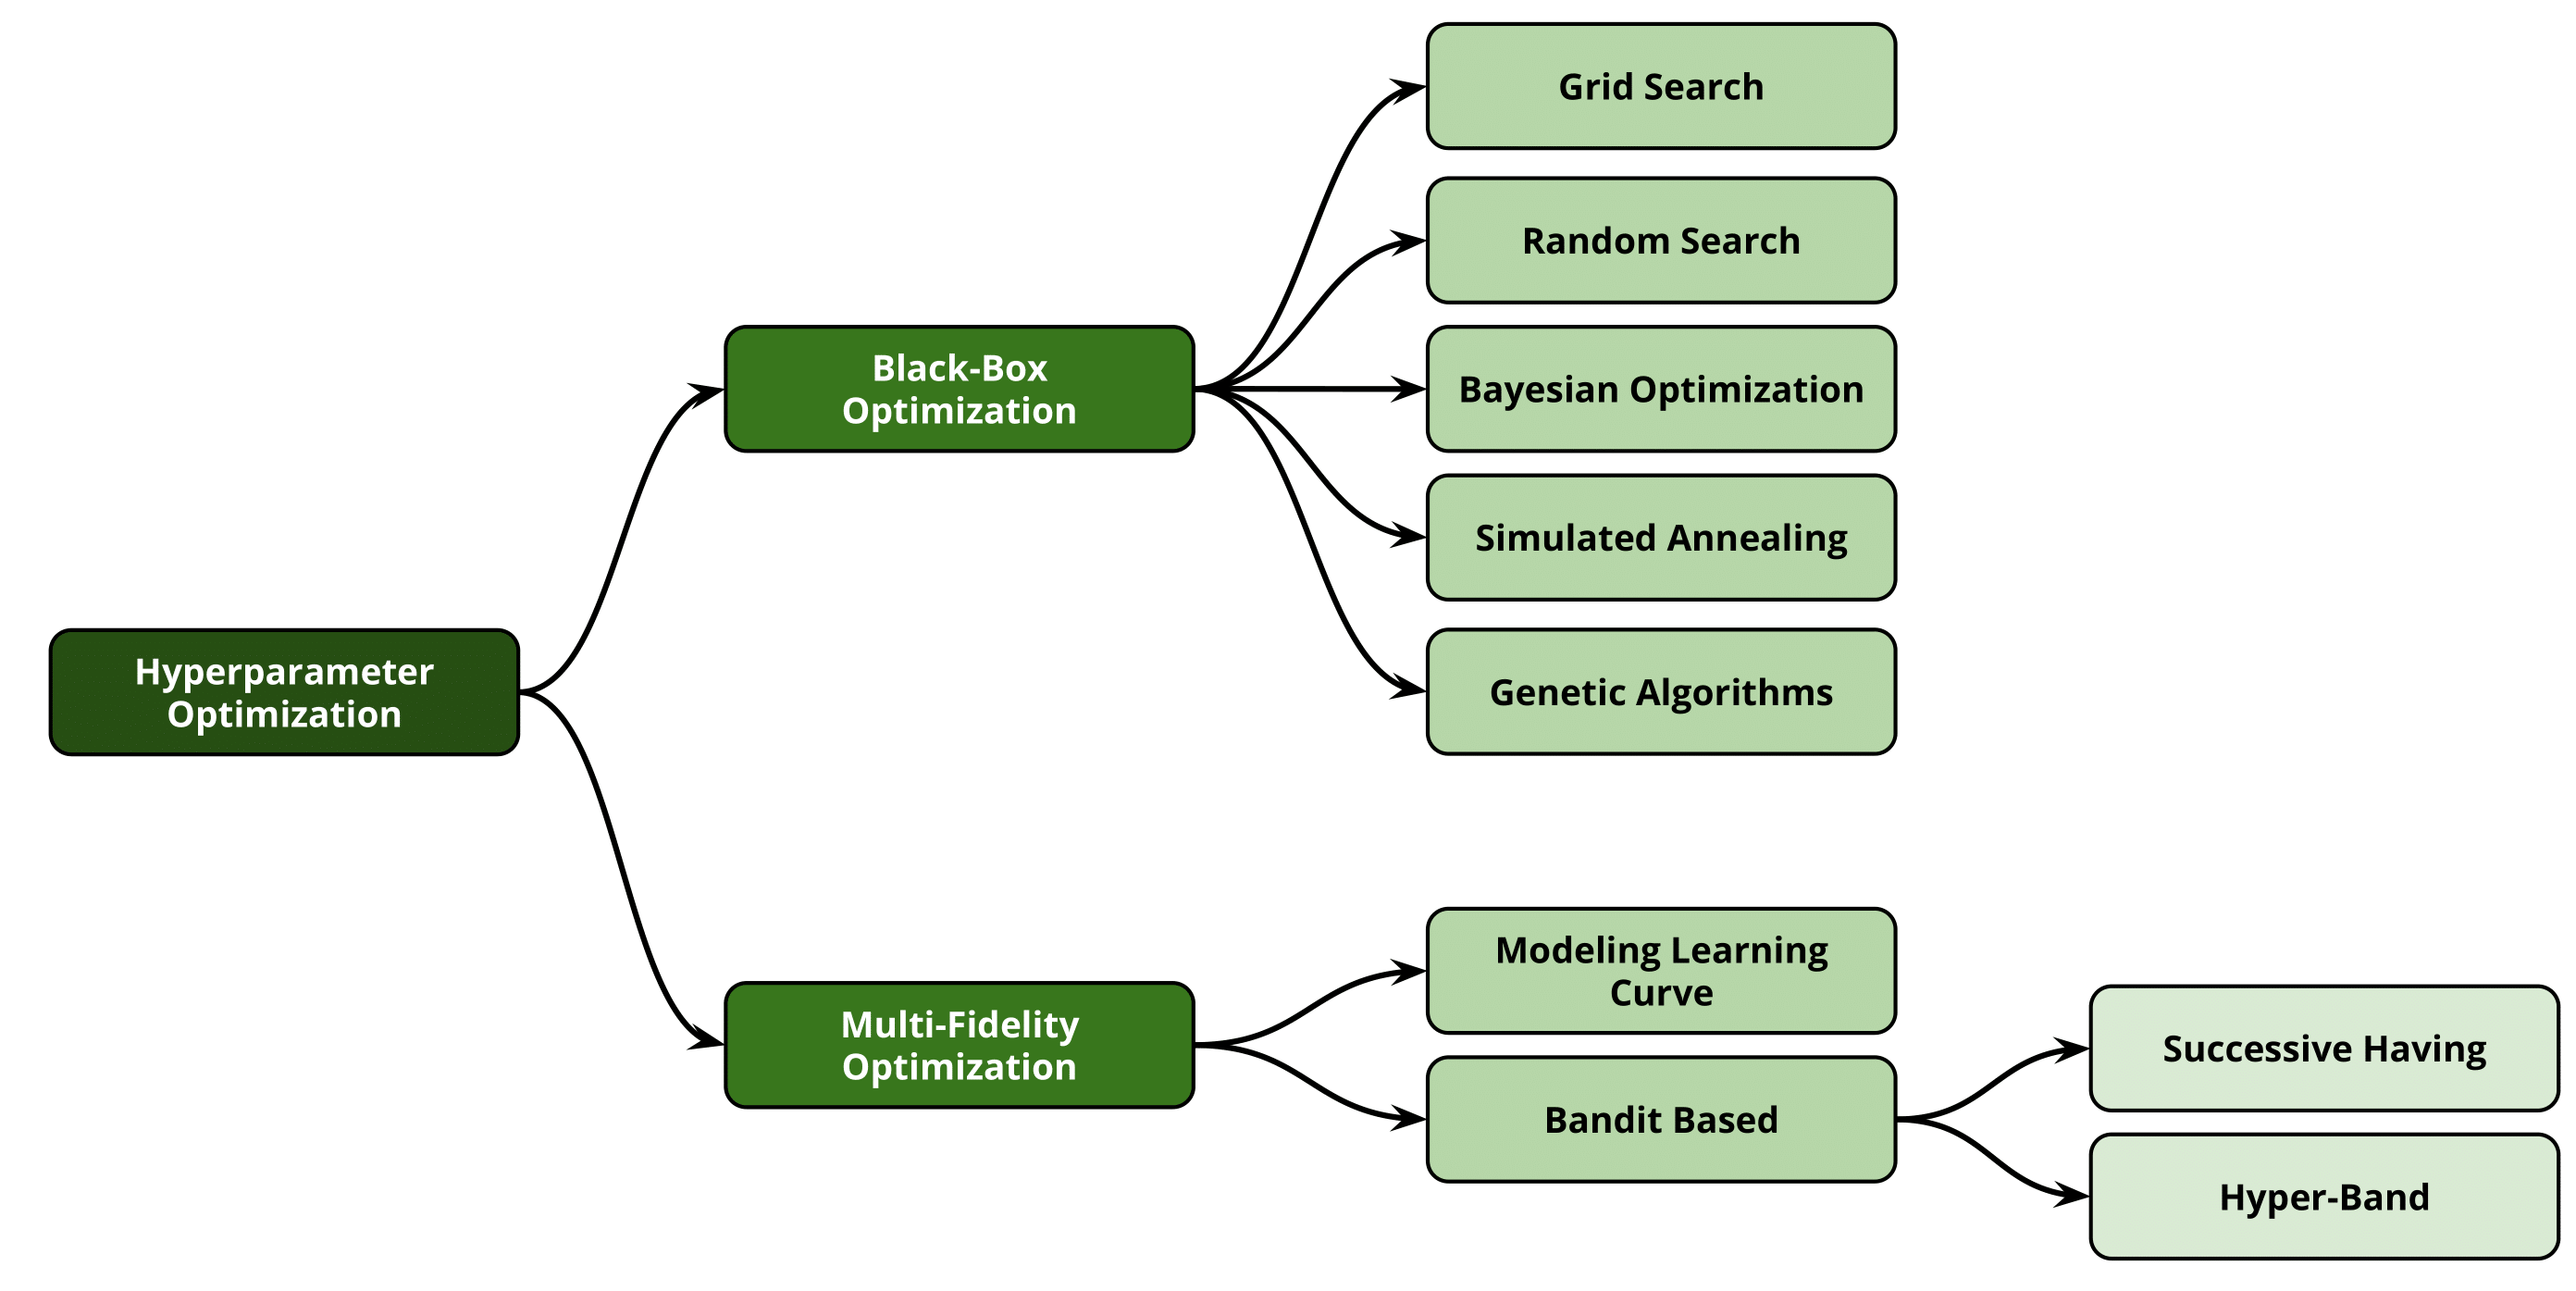
\includegraphics[width=\textwidth]{images/state_art-taxonomy_optimizers.png}
	\label{state_of_art:image:taxonomy}
	\caption{A Taxonomy for the Hyper-parameter Optimization Techniques \parencite{elshawi2019automated}.}
\end{figure}

\subsubsection{Black-Box Optimization Algorithms}

The 2 most common uninformed methods for \acrshort{hpo} are grid search and random search.
\todo{rewrite this to refer to blackbox optimization}

\paragraph{Grid Search}
Traditionally grid search is used for \acrshort{hpo} \parencite{liashchynskyi2019grid} wherehas a researcher or developer predefines possible values for a given hyperparameter and tests every hyper parameter combination from the solution space provided (see Figure \ref{grid}).

\begin{figure}[ht]
	\centering
	\begin{tikzpicture}
		\begin{axis}[
			title={Solution space for 2 hyper parameters},
		    xlabel={Hyper parameter $\alpha$},
		    ylabel={Hyper parameter $\beta$},
		    xmin=0, xmax=6,
		    ymin=0, ymax=6,
		    xtick={0,1,2,3,4,5},
		    ytick={0,1,2,3,4,5},
		    ymajorgrids=true,
		    xmajorgrids=true,
		    xticklabels={},
		    yticklabels={}
		]
		\addplot+[
			only marks,
		    mark options={color=lightblue},
		    mark=*,
		    mark size=2.9pt]
		    coordinates {
		    (0.5,0.5)(0.5,1)(0.5,1.5)(0.5,2)(0.5,2.5)(0.5,3)(0.5,3.5)(0.5,4)(0.5,4.5)(0.5,5)(0.5,5.5)
		    (1,0.5)(1,1)(1,1.5)(1,2)(1,2.5)(1,3)(1,3.5)(1,4)(1,4.5)(1,5)(1,5.5)
		    (1.5,0.5)(1.5,1)(1.5,1.5)(1.5,2)(1.5,2.5)(1.5,3)(1.5,3.5)(1.5,4)(1.5,4.5)(1.5,5)(1.5,5.5)
		    (2,0.5)(2,1)(2,1.5)(2,2)(2,2.5)(2,3)(2,3.5)(2,4)(2,4.5)(2,5)(2,5.5)
		    (2.5,0.5)(2.5,1)(2.5,1.5)(2.5,2)(2.5,2.5)(2.5,3)(2.5,3.5)(2.5,4)(2.5,4.5)(2.5,5)(2.5,5.5)
		    (3,0.5)(3,1)(3,1.5)(3,2)(3,2.5)(3,3)(3,3.5)(3,4)(3,4.5)(3,5)(3,5.5)
		    (3.5,0.5)(3.5,1)(3.5,1.5)(3.5,2)(3.5,2.5)(3.5,3)(3.5,3.5)(3.5,4)(3.5,4.5)(3.5,5)(3.5,5.5)
		    (4,0.5)(4,1)(4,1.5)(4,2)(4,2.5)(4,3)(4,3.5)(4,4)(4,4.5)(4,5)(4,5.5)
		    (4.5,0.5)(4.5,1)(4.5,1.5)(4.5,2)(4.5,2.5)(4.5,3)(4.5,3.5)(4.5,4)(4.5,4.5)(4.5,5)(4.5,5.5)
		    (5,0.5)(5,1)(5,1.5)(5,2)(5,2.5)(5,3)(5,3.5)(5,4)(5,4.5)(5,5)(5,5.5)
		    (5.5,0.5)(5.5,1)(5.5,1.5)(5.5,2)(5.5,2.5)(5.5,3)(5.5,3.5)(5.5,4)(5.5,4.5)(5.5,5)(5.5,5.5)
		    };
		\end{axis}
	\end{tikzpicture}
    \caption{Illustration of a grid search. The possible parameters are manually set and the algorithm does an exhaustive search on all the possible combinations.}
    \label{grid}
 \end{figure}

\paragraph{Random Search} This method is similar to grid search, but replaces manually set values with ranges and allows for randomized selection of hyper parameter values (see Figure \ref{random}). This method has been proven to be more efficient than grid search \parencite{JMLR:v13:bergstra12a}.

\begin{figure}[ht]
	\centering
	\begin{tikzpicture}
		\begin{axis}[
			title={Solution space for 2 hyper parameters},
		    xlabel={Hyper parameter $\alpha$},
		    ylabel={Hyper parameter $\beta$},
		    xmin=0, xmax=6,
		    ymin=0, ymax=6,
		    xtick={0,1,2,3,4,5},
		    ytick={0,1,2,3,4,5},
		    ymajorgrids=true,
		    xmajorgrids=true,
		    xticklabels={},
		    yticklabels={}
		]
		\addplot+[
			only marks,
		    mark options={color=lightblue},
		    mark=*,
		    mark size=2.9pt]
		    coordinates {
				(1.5,4)(2.5,4.1)(1.4,3)(1.6,3.6)(5.3,2.5)(5.4,2.3)(2.7,3.6)(1.5,5.1)(3.5,1.1)(3.1,5.7)(3.3,3.1)(3.5,1.8)(4.7,5.4)(3.7,2)(4.7,2.2)(2.7,2.4)(3.6,5.6)(2.5,5.9)(1.7,2.7)(4.1,5.9)
		    };
		\end{axis}
	\end{tikzpicture}
    \caption{Illustration of a random search. The hyper parameters values are randomly generated and the algorithm searches all the combinations.}
    \label{random}
 \end{figure}

\paragraph{Simulated Annealing}

This algorithm is based in the annealing process observed in metallurgy, where metal is heated to a high temperature and then slowly cooled, allowing for atoms in the metal to settle into more stable configurations \parencite{elshawi2019automated}.

Analogously, simulated annealing maintains a single candidate solution and takes steps of random size from the candidate in the search space, replacing the current candidate with a better solution or, with a certain probability, a worse one.

\paragraph{Bayesian Optimization}

Bayesian optimization can be described as sequential model-based optimization, whereas a probabilistic model is updated after every optimization attempt \parencite{dewancker}.

Various probabilistic regression can be used (e.g. Gaussian Processes and Random Forests). One of these regression models, Tree Parzen Estimators, deviates from the standard regression models, which use a predictive distribution $p(y|x)$. Instead, it creates two density functions that act as generative models for all domain variables \parencite{NIPS2011_86e8f7ab}\parencite{elshawi2019automated}.

\paragraph{Genetic Algorithms}

This set of optimization methods use algorithms inspired by biological evolution.

These algorithms are usually based on the idea of applying the multiple genetic operations (crossover, mutation, survival of the fittest) to a population of configurations \parencite{elshawi2019automated}.

\paragraph{Population-based Optimization}

This optimization technique is a hybrid of two methods of \acrshort{hpo}: random search and hand-tuning.

It starts by training a number of individual algorithms with random hyper parameters. But, instead of each algorithm working individually, they share information between them, to refine parameters and manage computational resources to solution sets that show promising results \parencite{jaderberg2017population}.

\subsubsection{Multi-Fidelity Optimization}

A area of increased attention in the\acrshort{hpo} research field is multi-fidelity techniques. These methods focus on decreasing the evaluation cost of a given function by combining cheap low-fidelity and expensive high-fidelity evaluations \parencite{elshawi2019automated}. These techniques are essential for optimization in high cost functions, where optimizing one hyperparameter can take days.

\paragraph{Bandit-based Optimization}

\todo{rewrite as a class of optimizers}
This technique is based on the \textit{multi-armed bandit problem}, whereas a limited set of resources must be allocated between competing choices, maximizing expected gain \parencite{Katehakis1987TheMB}. Similarly, using this algorithm in \acrshort{hpo} allows computers to stop execution of an algorithm (with defined hyper parameter values), by analyzing observable features during the run. This also leads to a decrease in computational power required to tune hyper parameters. \textit{Successive halving} is an example of an algorithm that employs this technique \parencite{jamieson2015nonstochastic}.

\subparagraph{HyperBand}

This algorithm is based on bandit-based optimization, solving the issue of time allocation in lieu of search time. As an example, \textit{successive halving} incurs on an issue regarding whether to allocate a large part of the time budget on exploring a large number of solutions rather than tuning a small number of them \parencite{elshawi2019automated}. \textit{HyperBand} attempts to solve this issue by partitioning the original time budget into smaller time and budget combinations and using \textit{successive halving} on each configuration \parencite{li2016hyperband}.

\todo{Successive Halving}

\subsubsection{Where are these supposed to go}

\paragraph{Gradient-based Optimization}

This algorithm uses the gradient of the model selection criterion with respect to the hyper parameters \parencite{bengio2000}. This algorithm is unsuitable when the optimizable function is treated as a black box function (where we only have access to  it's output and inputs).

\paragraph{Spectral Optimization}

This algorithm is inspired by techniques used in analysis of Boolean functions \parencite{hazan2017hyperparameter}. It specifically uses an iterative application of compressed sensing technique, allowing for easier parallelization.
